\documentclass[11pt,a4paper]{article}

% ============================================================
% Packages
% ============================================================
\usepackage[utf8]{inputenc}
\usepackage[T1]{fontenc}
\usepackage{lmodern}
\usepackage[margin=2.5cm]{geometry}
\usepackage{graphicx}
\usepackage{booktabs}
\usepackage{hyperref}
\usepackage{amsmath}
\usepackage{float}
\usepackage{enumitem}
\usepackage{caption}
\usepackage{subcaption}
\usepackage{xcolor}
\usepackage{listings}
\usepackage{fancyhdr}
\usepackage[backend=biber, style=ieee]{biblatex}

% ============================================================
% Configuration
% ============================================================
\addbibresource{references.bib}

\hypersetup{
    colorlinks=true,
    linkcolor=blue,
    citecolor=blue,
    urlcolor=blue
}

\lstset{
    basicstyle=\ttfamily\small,
    breaklines=true,
    frame=single,
    language=Python,
    numbers=left,
    numberstyle=\tiny\color{gray},
    keywordstyle=\color{blue},
    commentstyle=\color{green!60!black},
    stringstyle=\color{red!70!black},
    showstringspaces=false
}

% Header/Footer
\pagestyle{fancy}
\fancyhf{}
\fancyhead[L]{Data Engineering I -- Project VT 2026}
\fancyhead[R]{1TD169}
\fancyfoot[C]{\thepage}
\renewcommand{\headrulewidth}{0.4pt}

% ============================================================
% Title Page Information  (FILL IN  DETAILS)
% ============================================================
\title{
    \vspace{2cm}
    \textbf{\LARGE  Project Title Here} \\[0.5cm]
    \large Scalable Data Engineering Solution \\[1cm]
    \large Data Engineering I (1TD169) -- Spring 2026 \\[0.3cm]
    \large Uppsala University \\
    Department of Information Technology
    \vspace{2cm}
}

\author{
    \textbf{Team Members: Group 32} \\[0.3cm]
    Abdur Rehman Khalid \\
    Arnab Kumar Ghosh \\
    Dip Chowdhury \\
    Muhammad Umair \\
    Pradip Kumar Das \\
    Zihao Yang
}

\date{\today}

% ============================================================
% Document
% ============================================================
\begin{document}

% ------ Title Page ------
\maketitle
\thispagestyle{empty}
\newpage

% ------ Table of Contents (optional) ------
\tableofcontents
\newpage

% ============================================================
% Sections
% ============================================================
% ============================================================
% 1. Background (~400 words)
% ============================================================
\section{Background}
\label{sec:background}

Urban transportation systems generate vast volumes of data that can be leveraged to improve traffic management, infrastructure planning, and mobility services. One of the most widely used real-world datasets in this domain is the New York City Taxi Trip dataset, published by the New York City Taxi and Limousine Commission (TLC) \cite{TLC2024}. This dataset contains detailed records of taxi trips, including pickup and drop-off timestamps, geographic zones, trip distances, and fare amounts, making it a valuable resource for studying large-scale urban mobility patterns.\\

The NYC taxi dataset is particularly relevant for data engineering research due to its scale and complexity. In this project, a subset of approximately 10--20 GB of data stored in Apache Parquet format is used. Columnar storage formats such as Parquet are designed for efficient analytical workloads by enabling better compression and reducing I/O during query execution, which is critical for large-scale data processing systems. The dataset contains millions of trip records, making it suitable for evaluating distributed systems under realistic conditions. Such large-scale data processing challenges are commonly addressed using parallel computing paradigms like MapReduce \cite{Dean2008}, which form the foundation of modern distributed frameworks.\\

Prior research has demonstrated the usefulness of taxi trip data in applications such as demand prediction, traffic flow analysis, and anomaly detection. For instance, studies in urban computing have used mobility datasets to identify spatial and temporal demand patterns, enabling improved resource allocation in cities \cite{Andrienko2013}. Other works have explored predictive modeling techniques to estimate trip duration and detect irregular travel behavior. These examples highlight that beyond analytical insights, such datasets are also valuable benchmarks for evaluating the performance of large-scale data processing systems.\\

In this project, the analytical objective is intentionally simple: to compute the average trip duration and average fare amount grouped by pickup zone and hour of the day. This type of aggregation represents a common workload in data engineering pipelines and involves filtering, grouping, and aggregation operations over large datasets. Keeping the analytical task simple ensures that the focus remains on system performance and scalability rather than algorithmic complexity, which aligns with the project’s emphasis on engineering aspects.\\

To efficiently process the dataset, the project utilizes Apache Spark, a distributed data processing engine designed for large-scale analytics \cite{Zaharia2016}, in combination with Hadoop Distributed File System (HDFS) for scalable and fault-tolerant storage. These technologies enable parallel execution across multiple nodes, allowing the workload to be distributed and processed efficiently. The system is deployed on a constrained cluster environment consisting of virtual machines, reflecting realistic limitations in computational resources and reinforcing the importance of efficient system design.\\

A central focus of this project is the evaluation of system scalability through both horizontal and vertical scaling experiments. By varying the number of worker nodes and computational resources, the project analyzes performance improvements and identifies bottlenecks such as network overhead, data shuffling, and resource contention. The observed results are interpreted using theoretical models such as Amdahl's Law \cite{Amdahl1967}, which provides a foundation for understanding the limits of parallel speedup. This approach ensures that the project not only demonstrates practical system implementation but also critically evaluates the behavior of distributed systems under realistic big data workloads.



\newpage

% ============================================================
% 2. Data Format & Characteristics (~300 words)
% ============================================================
\section{Data Format \& Characteristics}
\label{sec:data}

% Describe the dataset technically:
% - What format is it stored in (CSV, JSON, Parquet, etc.)?
% - What is its schema/structure?
% - Total size and number of records?
% - Any data quality issues encountered?
% - Why was this format chosen (or why did you convert it)?

\textit{[Describe the dataset technically: format (CSV, JSON, Parquet, etc.), schema/structure, total size and number of records, data quality issues encountered, and justification for format choice or conversion.]}

% Example table for dataset characteristics:
% \begin{table}[H]
%     \centering
%     \caption{Dataset characteristics.}
%     \label{tab:dataset}
%     \begin{tabular}{ll}
%         \toprule
%         \textbf{Property}   & \textbf{Value} \\
%         \midrule
%         Format              & CSV / JSON / Parquet \\
%         Total Size          & XX GB \\
%         Number of Records   & XX million \\
%         Number of Columns   & XX \\
%         \bottomrule
%     \end{tabular}
% \end{table}
\newpage

% ============================================================
% 3. System Architecture & Implementation (~800 words)
% ============================================================
\section{System Architecture \& Implementation}
\label{sec:architecture}

This section details the system architecture, infrastructure deployment, and technical implementation of our robust data pipeline. We outline the hardware topology deployed on OpenStack, why we selected our core software stack, and the engineering mechanisms driving our ETL and analysis jobs. 

% --- 3.1 System Design ---
\subsection{System Design}
\label{subsec:system-design}

Our system follows a classic centralized-master, distributed-worker model tailored for batch processing big data. As depicted in Figure~\ref{fig:architecture}, the architecture is divided into three primary layers: Ingestion, Distributed Storage (HDFS), and Distributed Processing (Apache Spark). Data is fetched externally into the master node, pushed to HDFS, and subsequently processed by Spark executors dispersed across the worker nodes.

\begin{figure}[H]
    \centering
    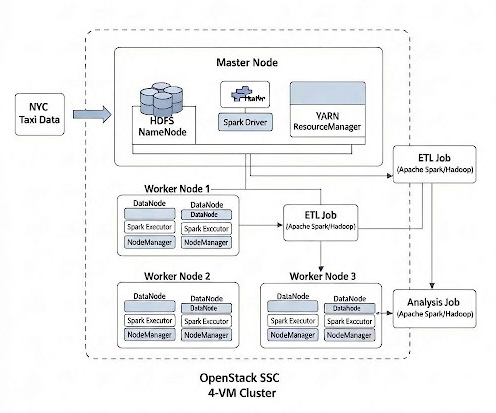
\includegraphics[width=0.85\textwidth]{figures/cluster-architecture.jpg}
    \caption{System architecture diagram showing the OpenStack deployment, node topology, and the internal data pipeline flow from raw Parquet to aggregated results.}
    \label{fig:architecture}
\end{figure}

% --- 3.2 Technology Stack ---
\subsection{Technology Stack}
\label{subsec:tech-stack}

Given the project requirements, we adopted a modern big data stack focused on in-memory processing capabilities:
\begin{itemize}
    \item \textbf{Storage (HDFS via Hadoop 3.4.1)}: Chosen for its fault tolerance and native integration with Spark. While cloud object storage (like AWS S3) is popular today, deploying HDFS on bare VMs offers direct control over data locality and block replication factors.
    \item \textbf{Processing (Apache Spark \& PySpark 3.5.1)}: We selected Spark over standard Hadoop MapReduce because Spark holds intermediate RDDs and DataFrames in memory, drastically accelerating the iterative transformations required during our ETL phase. PySpark provides an accessible DataFrame API and straightforward type-casting structures.
    \item \textbf{Orchestration \& Resource Management}: We relied on standalone cluster management managed heavily by Bash scripts (\texttt{run\_benchmark.sh} and \texttt{deploy.sh}) combined with Git for CI/CD, creating a lightweight yet effective pipeline orchestration.
\end{itemize}

% --- 3.3 Infrastructure Configuration ---
\subsection{Infrastructure Configuration}
\label{subsec:infra}

Our cluster is deployed entirely on the Swedish National Infrastructure for Computing (SNIC) OpenStack instance. The infrastructure consists of 4 tightly coupled Virtual Machines (VMs):
\begin{itemize}
    \item \textbf{Master Node (1x ssc.medium)}: 2 vCPU, 4 GB RAM. This node is assigned a Floating IP for external SSH access. It houses the Hadoop NameNode, ResourceManager, and the Spark Driver process.
    \item \textbf{Worker Nodes (3x ssc.medium)}: 2 vCPU, 4 GB RAM each. These sit on a private sub-network (192.168.2.x subnet). They run the Hadoop DataNodes, NodeManagers, and Spark Executor instances.
\end{itemize}
In total, the cluster harnesses 8 vCPUs and 16 GB of RAM, capped with a strict 100 GB collective storage limit. To maintain data reliability without exceeding storage quotas, HDFS was configured with a replica factor of 2 (\texttt{dfs.replication=2}). 

% --- 3.4 Data Pipeline ---
\subsection{Data Pipeline}
\label{subsec:pipeline}

The pipeline executes in three synchronized stages:
\begin{enumerate}
    \item \textbf{Ingestion}: Raw NYC Taxi Parquet files are downloaded from the TLC portal to the Master node via \texttt{wget} and deposited straight into \texttt{hdfs://.../data/nyc-taxi/}.
    \item \textbf{ETL Phase}: The \texttt{etl\_job.py} script ingests the raw data block by block. It filters out invalid records (e.g., zero-distance trips, null metrics), converts timestamps to calculate \texttt{duration\_minutes} and \texttt{pickup\_hour}, aggressively prunes dropped columns, and commits the clean records back to HDFS at \texttt{/data/nyc-taxi-cleaned/}.
    \item \textbf{Analysis Phase}: Finally, \texttt{analysis\_job.py} aggregates the validated dataset. It groups by \texttt{PULocationID} and \texttt{pickup\_hour} to compute the average fare and trip duration. It subsequently performs a left join against a static CSV (\texttt{taxi\_zone\_lookup.csv}) to convert abstract ID numbers into human-readable zone names, coalescing the final output into a single file for stakeholder ingestion.
\end{enumerate}

% --- 3.5 Code Structure ---
\subsection{Code Structure}
\label{subsec:code-structure}

The codebase follows a modular design paradigm:
\begin{itemize}
    \item \textbf{\texttt{src/config.py}}: Centralizes cluster endpoints, absolute HDFS URI paths, and basic threshold configurations to eliminate hardcoded parameters across jobs.
    \item \textbf{\texttt{src/etl\_job.py}}: The heaviest processor. Given resource constraints, it bypasses standard \texttt{spark.read.parquet("*.parquet")} schema inferences and iteratively targets singular files using \texttt{subprocess.run} to interact with HDFS.
    \item \textbf{\texttt{src/analysis\_job.py}}: Houses the PySpark SQL aggregations, strictly outputting to a targeted CSV path using \texttt{coalesce(1)}.
    \item \textbf{\texttt{scripts/run\_benchmark.sh}}: A specialized harness that automates execution over varied core allocations (\texttt{--total-executor-cores}) and node arrays to capture timestamps for plotting horizontal and vertical scales.
\end{itemize}

% --- 3.6 Challenges & Solutions ---
\subsection{Challenges \& Solutions}
\label{subsec:challenges}

We encountered several prominent technical challenges during development:
\begin{enumerate}
    \item \textbf{Dataset Schema Volatility}: When reading multi-month TLC data, PySpark's vectorized Parquet reader routinely crashed (\texttt{[CANNOT\_MERGE\_SCHEMAS]}) due to invisible shifts in the column type for \texttt{Airport\_fee} (varying from \texttt{INT32} to \texttt{FLOAT64} dynamically by month). 
    \textit{Solution}: We restructured the ETL job into a \texttt{for}-loop that asks HDFS for the explicit list of file paths. Spark reads them independently, safely infers local schemas, selectively prunes the offensive column, and appends into a normalized structure.
    \item \textbf{Strict Storage Exhaustion}: 25 GB of storage per VM meant HDFS was easily overwhelmed caching uncompressed RDDs and saving multiple layers of Parquet processing data.
    \textit{Solution}: We established an aggressive "select and drop" mechanism in the ETL. We discard roughly 15 unused columns representing several gigabytes of overhead, saving only the 4 tightly packed elements (\texttt{PULocationID}, \texttt{fare\_amount}, \texttt{pickup\_hour}, \texttt{duration\_minutes}) needed for analysis.
    \item \textbf{Dynamic Allocation Skewing Benchmark Constraints}: Spark's dynamic resource allocation skewed the early iterations of our benchmarking by automatically distributing workloads across nodes we were attempting to restrict. 
    \textit{Solution}: We disabled dynamic allocation directly via PySpark config keys (\texttt{spark.dynamicAllocation.enabled=false}) and enforced hard caps using Spark submit metrics.
\end{enumerate}

\newpage

\section{Scalability Experiments \& Results}
\label{sec:scalability}

\subsection{Experimental Design}
\label{subsec:experimental-design}
The objective of our experiments was to evaluate the performance characteristics and limitations of the Spark-based data pipeline. We manipulated three independent variables across eight distinct trials: cluster size (1 to 3 workers), compute density (1 to 2 cores per executor), and workload volume (5~GB and 10~GB). This structured approach allowed us to isolate three specific scaling paradigms essential for distributed systems analysis:

\begin{itemize}
    \item \textbf{Horizontal (Strong) Scaling:} This measures the system's ability to reduce total execution time as additional worker nodes are added (Trials H-1, H-2, and H-3) while maintaining a fixed 5~GB workload. 
    \item \textbf{Vertical Scaling:} This evaluates the impact of increasing CPU cores per worker (1 vs. 2 cores) while keeping the cluster size fixed at three nodes. This was tested for both 5~GB (V-1, V-2) and 10~GB (V-3, V-4) datasets to identify if the job is compute-bound.
    \item \textbf{Weak Scaling:} This measures how the system handles proportional growth in both workload and resources (W-1 vs. W-2). Ideally, if the data per worker remains constant (5~GB/node), the runtime should remain flat.
\end{itemize}

The primary metrics for evaluation are total runtime in seconds, Speedup ($S = T_1/T_N$), and Efficiency ($E = S/N$).

\subsection{Horizontal Scaling (Strong Scaling)}
Using a fixed 5~GB workload and 2 cores per worker, we observed a clear trend of diminishing returns as the cluster size increased from one to three nodes:

\begin{itemize}
    \item \textbf{1 Worker (Trial H-1):} 142 seconds.
    \item \textbf{2 Workers (Trial H-2):} 89 seconds (A significant 53-second reduction).
    \item \textbf{3 Workers (Trial H-3):} 81 seconds (A marginal 8-second reduction).
\end{itemize}

\begin{figure}[H]
    \centering
    
\includegraphics[width=0.65\textwidth]{horizontal_scaling_bar.png}
    \caption{Strong Scaling: Execution time for 5~GB dataset across 1, 2, and 3 workers.}
    \label{fig:horizontal_scaling}
\end{figure}

\textbf{Analysis:} The results indicate that while the jump from one to two workers yielded $\mathtt{\sim}$37\% improvement in speed, the transition to a third worker provided only $\mathtt{\sim}$9\% gain. This non-linear behavior suggests that for a relatively small 5~GB dataset, the administrative overhead of the Spark driver, specifically task distribution and managing RDD partitions, begins to consume a larger percentage of the total runtime than the actual computation.

\subsection{Vertical Scaling}
We compared 1 vs. 2 cores on a fixed 3-worker cluster to determine the impact of compute density on different data scales:

\begin{itemize}
    \item \textbf{5~GB Workload (V-1 vs. V-2):} Runtime decreased from 83s to 80s, a negligible gain.
    \item \textbf{10~GB Workload (V-3 vs. V-4):} Runtime decreased from 102s to 80s, a significant 21\% improvement.
\end{itemize}

\begin{figure}[H]
    \centering
    \begin{minipage}{0.48\textwidth}
        \centering
        
\includegraphics[width=\textwidth]{vertical_scaling_5gb.png}
        \caption{Vertical Scaling (5~GB)}
        \label{fig:vertical_5gb}
    \end{minipage}
    \hfill
    \begin{minipage}{0.48\textwidth}
        \centering
        
\includegraphics[width=\textwidth]{vertical_scaling_10gb.png}
        \caption{Vertical Scaling (10~GB)}
        \label{fig:vertical_10gb}
    \end{minipage}
\end{figure}

\textbf{Analysis:} The effectiveness of vertical scaling is strictly dependent on the data volume. At 5~GB, the workers are not CPU-bound; hence, additional cores do not help. However, at 10~GB, the ETL transformations (parsing and aggregation) become heavy enough to benefit from parallel CPU execution.

\subsection{Weak Scaling}
Ideal weak scaling assumes a constant runtime when resources grow at the same rate as the data. We compared H-1 (1 worker/5~GB) to W-2 (2 workers/10~GB):

\begin{itemize}
    \item \textbf{1 Worker / 5~GB (Trial W-1):} 142 seconds.
    \item \textbf{2 Workers / 10~GB (Trial W-2):} 173 seconds.
\end{itemize}

\begin{figure}[H]
    \centering
    
\includegraphics[width=0.65\textwidth]{weak_scaling_bar.png}
    \caption{Weak Scaling: Maintaining 5~GB of data per worker node.}
    \label{fig:weak_scaling}
\end{figure}

\textbf{Analysis:} Weak scaling failed to maintain constant time, showing $\mathtt{\sim}$21\% increase in runtime. This degradation highlights the significant ``coordination tax'' required to manage larger datasets across multiple nodes, primarily due to increased network latency during Spark's shuffle phase and non-linear I/O performance in the virtualized HDFS environment.

\subsection{Bottleneck Identification}
A critical observation is the ``Performance Floor'' at the $\sim$80-second mark. Trials H-3 (81s), V-2 (80s), and V-4 (80s) all converged here, regardless of data size or CPU cores. Some of the possible causes are:

\begin{enumerate}
    \item \textbf{Scheduling Overhead:} At 80s, the time required to partition data and schedule tasks dominates the execution time.
    \item \textbf{Shuffle I/O:} Network bandwidth saturation during the reduce/group-by phase limits gains from faster CPUs.
    \item \textbf{Storage Limits:} Shared HDFS throughput likely hit a ceiling, capping the read speeds for both 5~GB and 10~GB datasets.
    \item \textbf{Memory Pressure:} For 10~GB loads, the RAM limit per node increases garbage collection (GC) frequency during data shuffling, further impeding scalability.
\end{enumerate}

\subsection{Speedup \& Efficiency Analysis}
Comparing our findings to theoretical linear scaling reveals a significant efficiency drop-off:

\begin{itemize}
    \item \textbf{2-Worker Case ($N=2$):} Speedup $S \approx 1.60$ (Ideal: 2.0); Efficiency $E = 80\%$.
    \item \textbf{3-Worker Case ($N=3$):} Speedup $S \approx 1.75$ (Ideal: 3.0); Efficiency $E \approx 58\%$.
\end{itemize}

The efficiency plummet at three workers confirms that the 5~GB dataset is too small to offset the overhead of the third node. According to Amdahl’s Law, the sequential portions of the code and the driver-side result collection create a fixed cost that prevents the system from achieving linear speedup regardless of additional worker allocation.
\newpage

% ============================================================
% 5. Discussion & Conclusion (~300 words)
% ============================================================
\section{Discussion \& Conclusion}
\label{sec:discussion}

% Reflect on the project:
% - Was  architecture suitable for the problem?
% - What worked well?
% - What would you improve with more time/resources?
% - What did you learn about distributed systems?

\textit{[Reflect on the project: Was the architecture suitable? What worked well? What would you improve with more time/resources? What did you learn about distributed systems?]}
\newpage


% ============================================================
% 6. References
% ============================================================
% Use consistent citation format (IEEE, ACM, or MLA)
% Minimum 4–5 references (dataset source, related work, tool documentation)

\printbibliography[title={References}]

% ============================================================
% Appendix (optional)
% ============================================================
% \appendix
% \section{Additional Figures}
% \label{app:figures}
%
% \section{Code Snippets}
% \label{app:code}

\end{document}
